\documentclass[10pt]{article}
\usepackage{fancyhdr}
% \usepackage{ctex}
\usepackage{listings}
\usepackage[a4paper, body={16cm,24cm}]{geometry}
\usepackage{amsmath,amssymb,amstext,wasysym,enumerate,graphicx}
\usepackage{float,abstract,booktabs,indentfirst,amsmath}
\usepackage{multirow}
\usepackage{enumitem}
\usepackage{listings}
\usepackage{xcolor}
\usepackage{tabularx}
\usepackage[most]{tcolorbox}
\usepackage{accsupp}
\usepackage[bottom]{footmisc}
\usepackage{subcaption}
\usepackage{titlesec}
% \usepackage[backend=biber,style=numeric]{biblatex}
\usepackage[xetex]{hyperref}
\usepackage{setspace}
\setstretch{1.2}
\usetikzlibrary{arrows.meta}
\newcommand\emptyaccsupp[1]{\BeginAccSupp{ActualText={}}#1\EndAccSupp{}}
\setlength{\parindent}{2em}
\renewcommand\arraystretch{1.4}
% \setmonofont{Consolas}
% \setCJKmonofont{黑体}
% \setmainfont{Times New Roman}
\hypersetup{CJKbookmarks=true,colorlinks=true,citecolor=blue,%
            linkcolor=blue,urlcolor=blue,bookmarksnumbered=true,%
            bookmarksopen=true,breaklinks=true}
\lstset{
    % language = C,
    xleftmargin = 3em, 
    xrightmargin = 3em, 
    % aboveskip = 1em,
	backgroundcolor = \color{white}, % 背景色
	basicstyle = \small\ttfamily, % 基本样式 + 小号字体
	rulesepcolor= \color{gray}, % 代码块边框颜色
	breaklines = true, % 代码过长则换行
	numbers = left, % 行号在左侧显示
	numberstyle = \small\emptyaccsupp, % 行号字体
    % numbersep = -14pt, 
    keywordstyle=\color{purple}\bfseries, % 关键字颜色
    commentstyle =\color{red!50!green!50!blue!60}, % 注释颜色
    stringstyle = \color{red}, % 字符串颜色
    morekeywords={ASSERT, int64_t, uint32_t},
	% frame = shadowbox, % 用(带影子效果)方框框住代码块
    frame = single, % 用方框框住代码块
	showspaces = false, % 不显示空格
    showstringspaces = false,
	columns = fixed, % 字间距固定
    literate=
        {^+}{{{\color{black}\textbf{+}}\colorbox{green!30}{\phantom{XX}}}}1
        {+\t}{{{\color{black}\textbf{+}}\colorbox{green!30}{\phantom{XX}}}}1,
}

\raggedbottom

\title{Paper Summary of \textit{MapReduce: Simplified Data Processing on Large Clusters\footnote{Dean, Jeffrey, and Sanjay Ghemawat. ``MapReduce: simplified data processing on large clusters.'' \textit{Communications of the ACM} 51.1 (2008): 107-113.}}}
\author{Li, Pengda \\[-0.5em] \small{10225101460}}
\date{}

\begin{document}

\maketitle

\section{Background}

In early 2000s, with the rapid development of the Internet and distributed systems, processing large-scale data sets has become a common problem. 
Developers in Google and other companies implemented hundreds of special-purpose computations that process large amounts of raw data.
However, the input data is usually large that it must be calculated on a cluster of thousands of machines to complete in a reasonable time.
How to calculate in parallel, distribute the data and handle failures make the problem more complex.
Traditional methods struggled to handle this situation efficiently.
This hilighted the need for a new distributed computing model to solve these problems.  


\section{Main Problems}

\textit{Parallelization}. As the data is too large to be processed on a single machine, the computation must be parallelized to run on clusters. The model should provide a simple or automatic way to parallelize the computation.

\textit{Distribution}. To process efficiently, the data should be distributed across the machines. The model should handle the distribution of data and the scheduling of tasks.

\textit{Fault Tolerance}. When error occurs on a machine, the model should handle the error---either by trying to restart or by scheduling the task on another machine.

These problems undeniably exists and are important in distributed computing.
Parallelization is essential to break down computations and distribute them across machines.
However, efficient parallelization relies on proper distribution. 
Fault tolerance is also important to ensure the robustness of the system.
All of the three problems are important and should be addressed in a good designed distributed computing model.

\section{Model}

The authors proposed a new model called \textbf{MapReduce} to solve the problems above. 
Their inspiration came from the \textit{map} and \textit{reduce} functions in functional programming languages such as Lisp.
They use these two functions to describe a computation.

\subsection{\texttt{map}}

\texttt{map} function handles the input data and produces a set of intermediate key/value pairs. Each mapper processes a subset of the input data independently, which makes it easy to parallelize the computation. Type of the \texttt{map} function can be described as follows:

\begin{lstlisting}[numbers=none, frame=none, escapeinside={$$}{$$}, xleftmargin=0.3\textwidth, xrightmargin=0.3\textwidth]
map (k1, v1) $$$\rightarrow\ $$$ list(k2, v2)
\end{lstlisting}

The process of \texttt{map} is simple.
First, the input data is divided into splits.
Then each mapper processes one split with a user-defined logic, producing a set of intermediate key/value pairs.
In the end, the output is a combined set of all the key/value pairs produced by all mappers.

Take the program of counting words as an example. 
The program reads several documents as input data and counts the frequency of each word.
The \texttt{map} function reads each document and emits a key/value pair for each word in the document.
Figure \ref{fig:map} shows the pseudocode of it.

\begin{figure}[H]
\centering

\begin{lstlisting}[xleftmargin=0.3\textwidth, xrightmargin=0.3\textwidth]
map(String key, String value):
    // key: document name
    // value: document contents
    for each word w in value:
        EmitIntermediate(w, "1");
\end{lstlisting}
\caption{Pseudocode of the \texttt{map} function in word count program.}
\label{fig:map}
\end{figure}

The \texttt{map} function will produce a set of key/value pairs, such as \texttt{("apple", "1")}, \texttt{("banana", "1")}, etc.

\subsection{\texttt{reduce}}

The \texttt{reduce} function accept a key and a set of values for that key, which are produced by the \texttt{map} function. It merges the values. The type of the \texttt{reduce} function can be described as follows:

\begin{lstlisting}[numbers=none, frame=none, escapeinside={$$}{$$}, xleftmargin=0.3\textwidth, xrightmargin=0.3\textwidth]
reduce (k2, list(v2)) $$$\rightarrow\ $$$ list(v2)
\end{lstlisting}

The process of reduce is also simple. First, shuffle and sort the intermediate key/value pairs by key. Then each reducer receives a key and all values associated with it. Last, the reducer processes the key and values to generated the final output with a user-defined logic.

Take the word count example again. The \texttt{reduce} function sums the values for each word to get the final count. Figure \ref{fig:reduce} shows the pseudocode of it.

\begin{figure}[H]
\centering

\begin{lstlisting}[xleftmargin=0.29\textwidth, xrightmargin=0.28\textwidth]
reduce(String key, Iterator values):
    // key: a word
    // values: a list of counts
    int result = 0;
    for each v in values:
        result += ParseInt(v);
    Emit(AsString(result));
\end{lstlisting}

\caption{Pseudocode of the \texttt{reduce} function in word count program.}
\label{fig:reduce}
\end{figure}

The data it receives is like \texttt{("apple", ["1", "1", "1"])}, \texttt{("banana", ["1", "1"])}, etc. And the output is like \texttt{("apple", "3")}, \texttt{("banana", "2")}, etc.

\section{Implement}

There can be various ways to implement the MapReduce model. The authors provided a implementation of it that is widely used in Google.

\subsection{Execution Overview}

\begin{figure}
\centering
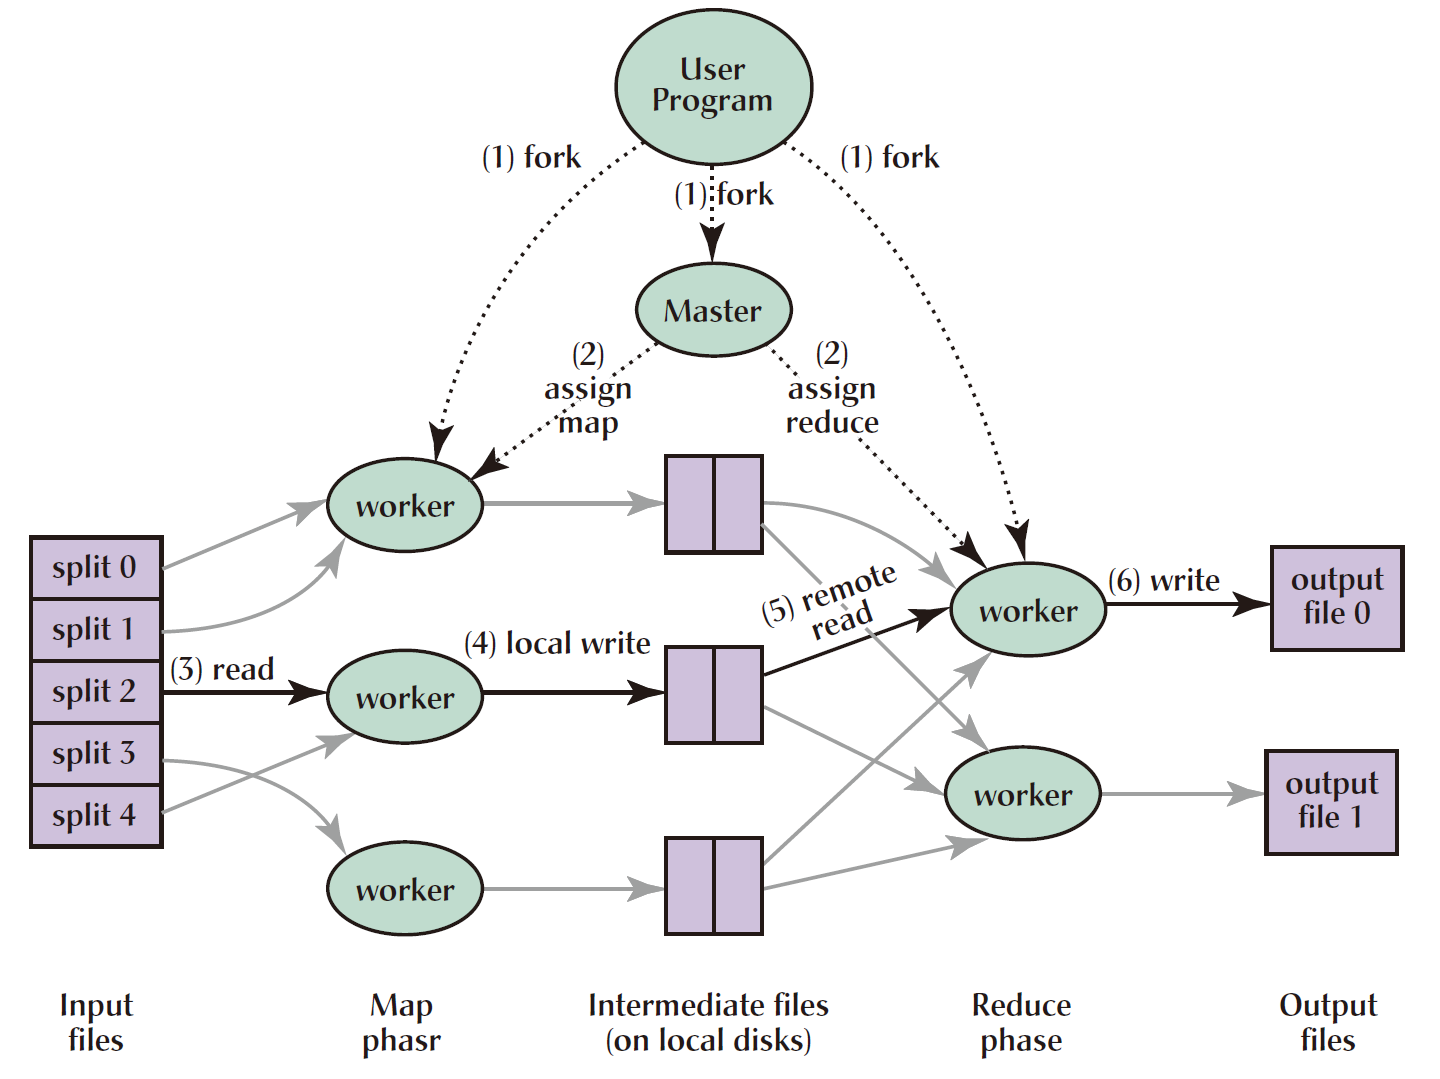
\includegraphics[width=0.7\textwidth]{img/1.png}
\caption{Execution overview of MapReduce.}
\label{fig:overview}
\end{figure}

Figure \ref{fig:overview} shows the overall flow of a MapReduce function. An execution process is as follows:

\begin{enumerate}
    \item Split the input files into $M$ pieces. Start up copies of the program on the machines in the cluster.
    \item Master, a special copy of the program, assigns $M$ map tasks and $R$ reduce tasks to the workers.
    \item A map worker reads the contents of the corresponding input split and applies the user-defined \texttt{map} function to the data. The intermediate key/value pairs are buffered in memory.
    \item Periodically, the buffered pairs are written to local disk, partitioned into $R$ regions and then it's location will be sent to master to forward to reduce workers.
    \item When a reduce worker is notified of the location of the intermediate data, it reads the data from the local disk and sorts it by key.
    \item For each unique key, the reduce worker applies the user-defined \texttt{reduce} function to it. The final output is written to the output file.
    \item When all map and reduce tasks are completed, the master wakes up the user program and returns.
\end{enumerate}

\subsection{Fault Tolerance}

The MapReduce model is designed to handle machine failures. 
The master node periodically monitors the workers. 
If a worker fails, the master will reassign the tasks to other workers. 
It also notifies relevant nodes to update task statuses accordingly.
This implements an efficient fault tolerance mechanism for large-scale worker node failures.

\section{Innovation}

The introduction of the MapReduce model is a significant innovation in the field of distributed computing since it greatly simplifies it.
Inspired by functional programming languages, MapReduce introduces two simple function abstractions, \texttt{map} and \texttt{reduce}, hiding the complexity of parallelization, distribution, and fault tolerance under the model.
Developers only need to focus on the \texttt{map} and \texttt{reduce} functions, instead of worrying about the underlying details of distributed computing.

From today's perspective, MapReduce is often regarded as one of the first widely used distributed computing frameworks, especially in the context of big data processing.
It also inspired many other distributed computing models, such as Apache Hadoop, Apache Spark, etc.

\section{Advantages}

\begin{itemize}
    \item \textbf{Simplicity}. MapReduce is simple and easy to understand. It makes it come true to parallelize and distribute computations on large clusters simply by defining two functions.
    \item \textbf{Scalability}. The model can be easily scaled to handle large-scale data of PB level. And we can expand it by just adding more machines to the cluster.
    \item \textbf{Fault Tolerance}. MapReduce can automatically detect failures and handle them. It ensures the robustness of the system.
\end{itemize}

\section{Disadvantages}

\begin{itemize}
    \item \textbf{High Latency}. Since the process of mapping, shuffling, sorting, and reducing takes time, the latency of the system is relatively high. It may not be suitable for real-time processing.
    \item \textbf{High Disk I/O}. As it shown in Figure \ref{fig:overview}, the intermediate data is written to disk and read from disk. This may cause high disk I/O. Since data is written and read from disk, it can not use the memory efficiently, which may cause performance issues.
\end{itemize}

\end{document}